\section{Theoretical Background}
\subsection{Definitions}


\subsubsection{Diffraction}
Diffraction is a purely wave-like phenomenon which cannot be modeled using the standard ray theory of light.
Interesting diffraction phenomena, however, occur mostly when the surface detail is highly anisotropic, viz. non-isotropic
Interference produces colorful effects due to the phase differences caused by a wave traversing thin media of different indices of refraction
Diffraction occurs when the surface detail is comparable to the wave- length of light


Light rays passing through a small aperture will begin to diverge and interfere with one another. This becomes more significant as the size of the aperture decreases relative to the wavelength of light passing through, but occurs to some extent for any aperture or concentrated light source.

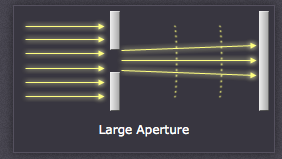
\includegraphics[scale=0.5]{images/1.png}
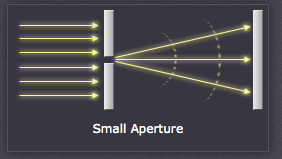
\includegraphics[scale=0.5]{images/2.png}

Since the divergent rays now travel different distances, some move out of phase and begin to interfere with each other — adding in some places and partially or completely canceling out in others. This interference produces a diffraction pattern with peak intensities where the amplitude of the light waves add, and less light where they subtract. If one were to measure the intensity of light reaching each position on a line, the measurements would appear as bands similar to those shown below.

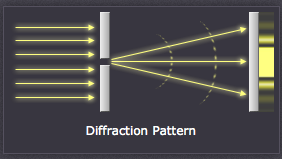
\includegraphics[scale=0.5]{images/3.png}

Diffraction refers to various phenomena which occur when a wave encounters an obstacle. In classical physics, the diffraction phenomenon is described as the apparent bending of waves around small obstacles and the spreading out of waves past small openings.

While diffraction occurs whenever propagating waves encounter such changes, its effects are generally most pronounced for waves whose wavelength is roughly similar to the dimensions of the diffracting objects. If the obstructing object provides multiple, closely spaced openings, a complex pattern of varying intensity can result. This is due to the superposition, or interference, of different parts of a wave that travels to the observer by different paths (see diffraction grating).

The effects of diffraction are often seen in everyday life. The most striking examples of diffraction are those that involve light; for example, the closely spaced tracks on a CD or DVD act as a diffraction grating to form the familiar rainbow pattern seen when looking at a disk

In optics, a diffraction grating is an optical component with a periodic structure, which splits and diffracts light into several beams travelling in different directions. The directions of these beams depend on the spacing of the grating and the wavelength of the light so that the grating acts as the dispersive element.

The relationship between the grating spacing and the angles of the incident and diffracted beams of light is known as the grating equation.

Fresnel and Frauenhofer diffraction
frauenhofer diffraction = infinite observation distance.
In multiple slit patterns each slit produces a diffraction pattern. Hence, multiple slit interference pattern is superimposed over single slit diffraction pattern.


\subsubsection{Radiometry}
Light is fundamentally a propagation form of enegry, so it is useful to define the SI unit of energy which is joule (J). To aid our intuituin let us describe radiometry in terms of collections of large numbers of photons. A photon can be considered as a quantum of light that has a position, direction of propagation and a wavelength $\lambda$ measured in nanometers. A photon has a speed c that depends only on the refractive index n of the medium through which it propagates, which allows us do define the frequency $f = \frac{c}{\lambda}$. The amount of energy q carried by a photon is given by the following relationship: $q = hf=  \frac{hc}{\lambda}$ where h is the Plank's constant.

\paragraph{Spectral Energy}
If there is a large collection of photons given, their total energy $Q = \sum_i q_i$ is the sum of each photon $q_i$. But how is the energy distributed across wavelenghts? One way in order to determine this distribution is to order all photons by their associated wavelength and then histogramming them, i.e. discretizing the spectrum and combine all photons which will fall into the same interval, i.e. compute the sum for each interval from the energy of all their photons. By dividing such an interval by its length,denoted as $Q_\lambda$, we get a relatively scaled interval energy energy, which is called sprectral energy and it is an intensive quantity. Intensive quantities can be though of as density functions that tell the density of an extensive quantity at an infinitesimal point.

\paragraph{Power}
Power is the estimated rate of energy production for light sources and is measured in the unit watts, denoted by Q, which is another name for joules per second. Since power is a density over time, it is well defined even when energy prodction is varying over time. As with enery, we are really intereded in spectral power, measured in W/nm, denoted as $\Phi_\lambda$

\paragraph{Irradiance}
The term irradiance comes into place when we are interested in how much light hits a given point. In order to answer this question, we must make use of a density function. Let $\delta A$ a fintie area sensor that is smaller than the light field being measured. The spectral irradiance H is just the power per unit area $\delta \frac{\Phi}{\delta A}$ which is $E = \frac{\delta q}{\delta A \delta t \delta \lambda}$ thus the units of irradiance are $Jm^{-2}s^{-1}(nm)^{-1}$

\paragraph{Radiance}

SHOW IMAGE: SOLID angle

$WIKI: http://en.wikipedia.org/wiki/Radiance$
$CG Slides 2012 - 6.shading$
$Book: Fundamentals of computer graphics$

Energy carried along a narrow beam of light

Although irradiance tells us how much lighjt is arriving at a point, it tells us little about the direction that light comes from. To measure something something similar to what we see with our eyes we need to be able to associate the quantity how much light with a specific direction. 

Radiance is a measure of the quantity of radiation that passes through or is emitted from a surface and falls within a given solid angle in a specified direction. This means radiance characterizes the total emission of reflectance. It indicates how much of the power emitted by an emitting or reflecting usrface will be receied by an optical system kooking at the surface from some angle of view.

think of light consisting of photon particles, each traeling along a ray. radiance is photon ray density, number of photons per area per solid angle.

Def $L = \frac{d^2 \Phi}{dA d\Omega cos(\theta)} \approx \frac{\Phi}{\Omega A cos(\theta)}$
where $L$ is the oberseved radiance in $Wm^-2 sr^-1$ in direction $\theta$, $\Theta$ is the total flux or power emitted, $\theta$ is the angle between the furface normal and the specified direction, A is the area of the surface and $\Omega$ is the solid angle in sr subtended by the observation or measurement.

Limit of energy passing through a small area in a small bundle of directions, divided by area and by solid angle spanned by bundle of directions, as area and solid angle get smaller.

Spectral radiance: energy at each wavelength
Units: energy per area per solid angle

\subsubsection{BRDF}
The bidirectional reflectance distribution function, in short BRDF, denoted as $f_r(w_i, w_r)$ is a four dimensional function that defines how light is reflected at an opaque surface. The function takes a negative incoming light direction, $\omega_{\text{i}}$, and outgoing direction, $\omega_{\text{r}}$, both defined with respect to the surface normal $\mathbf{n}$ and returns the ratio of reflected radiance exiting along $\omega_{\text{r}}$ to the irradiance incident on the surface from direction $\omega_{\text{i}}$
  
\begin{align}
  f_r(w_i, w_r)
  & = \frac{dL_r(w_r)}{dE_i(w_i)} \\
  & = \frac{dL_r(w_r)}{L_i(w_i)cos(\theta_i)dw_i}
\end{align}

where L is radiance, or power per unit solid-angle-in-the-direction-of-a-ray per unit projected-area-perpendicular-to-the-ray, E is irradiance, or power per unit surface area, and $\theta_{\text{i}}$ is the angle between $\omega_{\text{i}}$ and the surface normal, $\mathbf n$. The index $\text{i}$ indicates incident light, whereas the index $\text{r}$ indicates reflected light.

The reason the function is defined as a quotient of two differentials and not directly as a quotient between the undifferentiated quantities, is because other irradiating light than $\operatorname dE_{\text{i}}(\omega_{\text{i}})$, which are of no interest for $f_{\text{r}}(\omega_{\text{i}},\, \omega_{\text{r}})$, might illuminate the surface which would unintentionally affect $L_{\text{r}}(\omega_{\text{r}})$, whereas $\operatorname dL_{\text{r}}(\omega_{\text{r}})$ is only affected by $\operatorname dE_{\text{i}}(\omega_{\text{i}})$.

\subsubsection{Spectral Rendering}
In Computer Graphics, spectral rendering is where a scene's light transport is modeled considering the whole span of wavelengths instead of R,G,B values (still relating on geometric optic, which ignore wave phase). The motivation is that real colors of the physical world are spectrum; trichromatic colors are only inherent to Human Visual System.

\paragraph{CIE color spaces}
CIE 1931 RGB and CIE 1931 XYZ color spaces are the first mathematically defined color spaces. They were created by the International Commission on Illumination (CIE) in 1931.

The CIE's color matching functions $\overline{x}(\lambda)$, $\overline{y}(\lambda)$ and $\overline{z}(\lambda)$ are the numerical description of the chromatic response of the observer (described above). They can be thought of as the spectral sensitivity curves of three linear light detectors yielding the CIE tristimulus values X, Y and Z. Collectively, these three functions are known as the CIE standard observer.[9]

The tristimulus values for a color with a spectral power distribution $I(\lambda)$, are given in terms of the standard observer by:

    $X= \int_{380}^{780} I(\lambda)\,\overline{x}(\lambda)\,d\lambda$
    $Y= \int_{380}^{780} I(\lambda)\,\overline{y}(\lambda)\,d\lambda$
    $Z= \int_{380}^{780} I(\lambda)\,\overline{z}(\lambda)\,d\lambda$

where $\lambda$, is the wavelength of the equivalent monochromatic light (measured in nanometers).


\subsubsection{Signal}
A signal is a function that conveys information about the behavior or attributes of some phenomenon.
In the physical world, any quantity exhibiting variation in time or variation in space (such as an image) is potentially a signal that might provide information on the status of a physical system, or convey a message between observers

\subsubsection{Fourier Transformation}
The Fourier-Transform is a mathematical tool which allows to transform a given function or rather a given signal from defined over a time- (or spatial-) domain into its corresponding frequency-domain.
 
Let $f$ an measurable function over $\mathcal{R}^n$. Then, the coninious Fourier Transformation, denoted as FT, $\mathcal{F}\{t\}$ of $f$ is defined as, ignoring all constant factors in the formula:
 
\begin{equation}
  \mathcal{F}\{w\}_{FT} = \int_{\mathcal{R}^n} f(x)e^{-iwt} dt
\end{equation}

whereas its inverse transform is defined like the following which allows us to obtain back the original signal:

\begin{equation}
  \mathcal{F}\{w\}^{-1}_{FT} = \int_{\mathds{R}} \mathcal{F}\{w\}e^{iwt} dt
\end{equation}

By using fourier analysis, which is the approach to approximate any function by sums of simpler trigonometric functions, we gain the so called discrete time fourier transform (in short DTFT). The DTFT operates on a discrete function. Usually, such an input function is often created by diitally sampling a continius function. The DTFT itself is operation on a discretized signal on a continious, periodic frequency domain and looks like the following:

\begin{equation}
  \mathcal{F}\{w\}_{DFT} = \sum_{-\infty}^{\infty} f(x) e^(-iwk)
\end{equation}

we can further discretize the frequency domain and will get then the discrete fourier transformation (in short DFT) of the input signal:
\begin{equation}
  \mathcal{F}\{w\}_{DFT} = \sum_{n=0}^{N-1} f(x) e^(-iw_{n}k)
\end{equation}
Where the angular frequency $w_n$ is defined like the following $w_n = \frac{2\pi n}{N}$ and N is the number of samples within an equidistant periode sampling.

\subsubsection{Convolution}

\begin{equation}
  \mathcal (f*g)(t) = \int_{\mathcal{R}^n} f(t)g(t-x) dx
\end{equation}

Note that the Fourier transform of the convolution of two functions is the product of their Fourier transforms. This is equivalent to the fact that Convolution in spatial domain is equivalent to multiplication in frequency domain. Therefore, the inverse Fourier transform of the product of two Fourier transforms is the convolution of the two inverse Fourier transforms


\subsubsection{Taylor Series}
Taylor series is a representation of a function as an infinite sum of terms that are calculated from the values of the function's derivatives at a single point.

The Taylor series of a real or complex-valued function ƒ(x) that is infinitely differentiable at a real or complex number a is the power series:
\begin{equation}
  \mathcal T(f;a)(x) = \sum_{n=0}^{\infty} \frac{f^{n}(a)}{n!}(x-a)^n
\end{equation}


\subsection{Thesis Basis: J.Stam's Paper about Diffraction Shader}
GOAL
main task in the theory of diffraction is to solve this wave equation for different geometries.
we are interested in computing the reflected waves from various types of surfaces

abstract:
before: most reflection models empirically or based on ray-theory of light.
now: new reflection model based on wave theory modeling the effect of diffraction


In his Paper Diffraction Shader, Jos Stam derives a BRDF which modeling the effect of diffraction for various analytical anistropic reflaction models using the scalar Kirchof theory and the theory of random processes. By employing the so called scalar wave theory of diffraction [source 5 in stams paper] in which a wave is assumed to be a complex valued scalar. It's noteworthy, that stam's BRDF formulation does not take into account the polarization of the light. Fortunately, light sources like sunlight and light bulbs are unpilarizaed. In our simulations we will always assume we have given i directional light source, i.e. sunlight. Hence, we can use stam's model for our derivations

A further assumption in Stam's Paper is, the emanated waves from the source are stationary, which implies the wave is a superposition of independent monochromatic waves. This implies that each wave is associated to a definite wavelangth lambda. However, sunlight once again fulfills this fact.

Mention Helmolth equation, which has the solution $k = \frac{2\pi}{\lambda}$ which is the wavenumber


Based on his these previous assumptions and applying Stam starts his derviations by applying the so called Kirchhoff integral, which is relating the reflected field to the incoming field. This equation is a formalization of Huygen’s well-known principle that states that if one knows the wavefront at a given moment, the wave at a later time can be deduced by considering each point on the first wave as the source of a new disturbance, i.e. once the field  $\psi_1 =  e^{ik\mathbf{x} \cdot \mathbf{s}\mathbf{s}}$ on the surface is known, the field everywhere $\psi_2$ else away from the surface can be computed.
More precisely, we want to compute the wave $\psi_2$ equal to the reflection of an incoming planar monochromatic wave $\psi_1 = e^{ik k_1 * x}$  traveling in the direction $k_1$ from a surface S. Mathematically this can be formulized the following:

\begin{equation}
  \psi_2 = \frac{i k e^{i K R}}{4 \pi R}(F\mathbf{v}-\mathbf{p}) \cdot \int_{S} \hat{\mathbf{n}} e^{ik\mathbf{v} \cdot \mathbf{s} d\mathbf{s}}
\end{equation}


In applied optics, when dealing with scattered waves, one does use differential scattering cross-section rather than defining a BRDF which has the following identitiy: 

\begin{equation}
    \sigma^0 = 4 \pi \lim_{R \to \infty} R^2 \frac{\langle \left|\psi_2\right|^2\rangle}{\langle \left|\psi_1\right|^2\rangle}
\end{equation}

Relationship between the BRDF and the scattering cross section is the follwing:

The relationship between the BRDF and the scattering cross section can be shown to be equal to $BRDF = \frac{1}{4\pi}\frac{1}{A}\frac{\sigma^0}{cos(\theta_1)cos(\theta_2)}$
Wheras $\theta_1a$ and $\theta_2$ are the angles that the vectors $\hat{k_1}$
and $\hat{k_2}$ make with the vertical direction.
 
ADD FIGURE for k1, k2

where R is the disance from the center of the patch to the receiving point $x_p$, $\hat{\mathbf{n}}$ is the normal of the surface at s and the vectors:

\begin{equation*}
    \mathbf{v} = \hat{\mathbf{k_1}} - \hat{\mathbf{k_1}}
               = (u,v,w)
\end{equation*}

\begin{equation*}
    \mathbf{p} = \hat{\mathbf{k_1}} + \hat{\mathbf{k_1}}
\end{equation*}


During his derivations, Stam provides a analytical representation for the Kirchhoff integral by using his assumptions. He restricts himself to the reflaction of waves from height fields $h(x,y)$ with the assumption that the surface is defined as an elevation over the (x,y) plane using the surface plane approximation.

Which will lead him to the follwoing identity for the Kirchhoff integral

\begin{equation}
    \mathbf{I}(ku, kv) = \int \int \frac{1}{ikw}(-p_x, -p_y, ikwp) 
\end{equation}

wheras stam formulates for a hightfield auxilary function $p(x,y) = e^{iwkh(x,y)}$ where $w = -(cos(\theta_i)+cos(\theta_r))$ and $\theta_i$ and $\theta_r$ are the angles of incident and reflected directions with the surface normal (ADD picture) and the wavenumber $k=\frac{2\pi}{\lambda}$

\begin{equation}
    p(x,y) = e^{ikwh(x,y)}
\end{equation}

We the observation that the integral is a Fourier transform by $-iku$ and $-ikv$
which will lead us to his final derivation, using the identity of BRDF, and computing the limes:

\begin{equation}
    BRDF_{\lambda}(w_i, w_r) = \frac{k^2 F^2 G}{4\pi^2 A w^2} \langle \left|P(ku, kv)\right|^2\rangle
\end{equation}

$BRDF_{\lambda}(w_i, w_r)$ is BRDF where wavelength $\lambda$ $w_i$ and $w_r$ are incident and reflected normalized directions vectors, pointing away from the given surface. Which can be written, using the fourier transform (FT) $P(u,v) = F(p)(u,v)$, as:
$BRDF_{\lambda}(w_i, w_r) = \frac{F^2 G}{\lambda^2 A w^2}abs(P(\frac{u}{\lambda},\frac{v}{\lambda}))^2$ where F represents the Fresnel term, uv,v,w are derived from the incident and reflected directions as $(u,v,w) = -\omega_i - \omega_r$, abs(P) represents the expected valuess of a random variable X and A is an area of integration on the surface that is considered to contribute to diffraction, G is the geometry term which is $G   =\frac{(1-\hat{\mathbf{k_1}}\cdot\hat{\mathbf{k_2}})^2}{cos(\theta_1)cos(\theta_2)}$

and P(x,y) is the Fourier transform (FT) of the function p(x,y) from above.
This identitiy for the BRDF is the starting point for our derivations.


\subsection{Derivations}
\subsubsection{BRDF formulation}

EXPLAIN: Why do we want a formulation for $L_{\lambda}(w_r)$ in some words. what does it represent?

Definition of $BRDF(w_i, w_r) := f_r(w_i, w_r) = \frac{dL_r(w_r)}{dE_i(w_i)}=\frac{dL_r(w_r)}{L_i(w_i)cos(\theta_i)dw_i}$  
Hence, we can dervie the following expression:
\begin{align*}
f_r(w_i, w_r) = \frac{dL_r(w_r)}{L_i(w_i)cos(\theta_i)dw_i} \\
=> f_r(w_i, w_r) L_i(w_i)cos(\theta_i)dw_i = dL_r(w_r) \\
=> \int_{\Omega}f_r(w_i, w_r) L_i(w_i)cos(\theta_i)dw_i = \int_{\Omega}dL_r(w_r) \\
=> L_r(w_r) = \int_{\Omega}f_r(w_i, w_r) L_i(w_i)cos(\theta_i)dw_i
\end{align*}

We assume, that our incident light is a directional light source like sun-light and therefore its radiance is given as $L_{\lambda}(w)=I(\lambda)\delta(w-w_i)$ where $I(\lambda)$ is the intensity of the relative spectral power for the wavelength $\lambda$. Thus we get for our the brdf formulation:

\begin{align}
L_{\lambda}(w_r) 
& = \int_{\Omega} BRDF_{\lambda}(w_i, w_r) L_{\lambda}(w_i) cos(\theta_i) dw_i \\
& = BRDF_{\lambda}(w_i, w_r) I(\lambda) cos(\theta_i)
\end{align}

where $w_i$ is the solid angle for the incoming light, $\theta{_i}$ is the angle of incidence,
$w_r$ is the solid angle for the reflected light, $\lambda$ wavelength, $\Omega$ is the hemisphre we of integration for the incomming light.
Radiance reflected by given surface in given direction:
$L_{\lambda}(w_i)$ is the incomming radiance, $L_{\lambda}(w_r)$ is the reflected radiance

For the $BRDF(w_i, w_r)$ we are going to use the formulation dervied by Stam described above which looks like this using the fact that wavenumber $k=\frac{2\pi}{\lambda}$:

\begin{align*}
BRDF(w_i, w_r) 
& = \frac{k^2 F^2 G}{4\pi^2 A w^2} \langle \left|P(ku, kv) \right|^2\rangle \\
& = \frac{k^2 F^2 (1-\hat{\mathbf{k_1}}\cdot\hat{\mathbf{k_2}})}{cos(\theta_1)cos(\theta_2) 4\pi^2 A w^2} \langle \left|P(ku, kv)  \right|^2\rangle \\
& = \frac{4 \pi^2 F^2 (1-\hat{\mathbf{k_1}}\cdot\hat{\mathbf{k_2}})}{cos(\theta_1)cos(\theta_2) 4\pi^2 A \lambda^2 w^2} \langle \left|P(ku, kv)  \right|^2\rangle \\
& = \frac{F(w_i, w_r)^2 (1-\hat{\mathbf{k_1}}\cdot\hat{\mathbf{k_2}})}{cos(\theta_1)cos(\theta_2) A \lambda^2 w^2} \langle \left|P(ku, kv)  \right|^2\rangle
\end{align*}

where $\hat{\mathbf{k_t}}$ represents a unit vector whose spherical coordinates are given by the solid angle $t$.
Since we are going to integrate over a sphere $\Omega$ we can write the component $w=(cos(\theta_i)+cos(\theta_r))$
SHOW WHY WE ARE ALLOWED TO WRITE IT LIKE THIS => SPHERICAL COORDINATES DIFFERENCE $(k1 - k2) = (u,v,w)$ and so on.
this our identity for $L_{r}(w_r)$ will lead us to the following identiy using our identity :

\begin{align*}
L_{\lambda}(w_r) 
& = \frac{F(w_i, w_r)^2 (1-\hat{\mathbf{k_1}}\cdot\hat{ \mathbf{k_2}})^2}{A \lambda^2 cos(\theta_i)cos(\theta_r)  (cos(\theta_i)+cos(\theta_r))^2} \langle \left|P_{cont}(\frac{2\pi u}{\lambda}, \frac{2\pi v}{\lambda})  \right|^2\rangle cos(\theta_i) I(\lambda) \\
& = I(\lambda) \frac{F(w_i, w_r)^2 (1-\hat{\mathbf{k_1}}\cdot\hat{\mathbf{k_2}})^2}{\lambda^2 A (cos(\theta_i)+cos(\theta_r))^2 cos(\theta_r)} \langle \left|P_{cont}(\frac{2\pi u}{\lambda}, \frac{2\pi v}{\lambda})  \right|^2\rangle \\
& = I(\lambda) \frac{F(w_i, w_r)^2 (1-\hat{\mathbf{k_1}}\cdot\hat{\mathbf{k_2}})^2}{\lambda^2 A (cos(\theta_i)+cos(\theta_r))^2 cos(\theta_r)} \langle \left|T_0^2 P_{dtft}(\frac{2\pi u}{\lambda}, \frac{2\pi v}{\lambda})  \right|^2\rangle
\end{align*}

$P_{cont}$ is the continious inverse Fourier transform for the taylor seies of our hight-field representing the nano structure, i.e. $P(k,l) = \mathcal{F}^{-1}\{p\}(k,l)$ and $P_{dtft}$ is the dicrete-time inverse Fourier Transform for the same problem domain and $T_0$ the sampling distance for the discretization pf $p(x,y)$ assuming equal and uniform sampling in both dimensions $x,y$.



\subsubsection{Relative BRDF}
reason why relative brdf: In order to scale the reflactiance such that we are able to texture. 
convex combination reflectance with texture. Scale illumination.

Let us examine what $L_\lambda(w_r)$ will be for $w_r = w_0 := (0,0,*)$ i.e. specular reflection case, denoted as $L_\lambda^{spec}(w_0)$. 
When we know the expression for $L_\lambda^{spec}(w_0)$ we would be able to compute the relative reflected radiance for our problem by simply dividing $L_\lambda(w_r)$ by $L_\lambda^{spec}(w_0)$, denoted as 

\begin{equation}
    \rho_\lambda(w_i,w_r) = \frac{L_\lambda(w_r)}{L_\lambda^{spec}(w_0)}
\end{equation}

But first, let us derive the following expression:

\begin{align*}
L_\lambda^{spec}(w_0) 
& = I(\lambda) \frac{F(w_0, w_0)^2 (1-\colvec[0]{0}{1}\cdot\colvec[0]{0}{-1})^2}{\lambda^2 A (cos(0)+cos(0))^2 cos(0)} \langle \left|T_0^2 P_{dtft}(0,0)  \right|^2\rangle \\
& = I(\lambda) \frac{F(w_0, w_0)^2 (1+1)^2}{\lambda^2 A (1+1)^2 1}\left| T_0^2 N_{sample} \right|^2 \\
& = I(\lambda) \frac{F(w_0, w_0)^2}{\lambda^2 A}\left| T_0^2 N_{sample} \right|^2 
\end{align*}

Where $N_{samples}$ is the number of samples of the dtft.

Thus, we can plug our last derived expression into the definition for the relative reflectance radiance in the direction $w_r$ and will get:

\begin{align*}
\rho_\lambda(w_i,w_r)
& = \frac{L_\lambda(w_r)}{L_\lambda^{spec}(w_0)} \\
& = \frac{I(\lambda) \frac{F(w_i, w_r)^2 (1-\hat{\mathbf{k_1}}\cdot\hat{\mathbf{k_2}})^2}{\lambda^2 A (cos(\theta_i)+cos(\theta_r))^2 cos(\theta_r)} \langle \left|T_0^2 P_{dtft}(\frac{2\pi u}{\lambda}, \frac{2\pi v}{\lambda})  \right|^2\rangle}{I(\lambda) \frac{F(w_0, w_0)^2}{\lambda^2 A}\left| T_0^2 N_{sample} \right|^2 } \\
& = \frac{F^2(w_i,w_r)(1-\hat{\mathbf{k_1}}\cdot\hat{\mathbf{k_2}})^2}{F^2(w_0,w_0)(cos(\theta_i)+cos(\theta_r))^2 cos(\theta_r)}  \langle \left|\frac{P_{dtft}(\frac{2\pi u}{\lambda}, \frac{2\pi v}{\lambda})}{N_{samples}}\right|^2\rangle
\end{align*}

for simplification and a better overview, let us introduce the following expression, the so called gain factor

\begin{equation}
    C(w_i,w_r) = \frac{F^2(w_i,w_r)(1-\hat{\mathbf{k_1}}\cdot\hat{\mathbf{k_2}})^2}{F^2(w_0,w_0)(cos(\theta_i)+cos(\theta_r))^2 cos(\theta_r) N_{samples}^2}
\end{equation}

Using this substitute, we will end up with the following expression for the relative reflectance radiance

\begin{equation}
\rho_\lambda(w_i,w_r) =  C(w_i,w_r) \langle \left|P_{dtft}(\frac{2\pi u}{\lambda}, \frac{2\pi v}{\lambda})\right|^2\rangle
\end{equation}

using the previous definition for the relative reflectance radiance $\rho_\lambda(w_i,w_r) = \frac{L_\lambda(w_r)}{L_\lambda^{spec}(w_0)}$ which we can rearrange to the expression 

\begin{equation}
L_\lambda(w_r) = \rho_\lambda(w_i,w_r)L_\lambda^{spec}(w_0)
\end{equation}

Let us choose $L_\lambda^{spec}(w_0) = S(\lambda)$ such that is has the same pforifle as the relative spectral power distribuation of CIE Standard Illuminant $D65$. Further, when integration over $\lambda$ for a specular surface we should get $CIE_XYZ$ values corresponding to the white point for $D65$ 

the corresponding tristimulus values using CIE colormatching functions for the $CIE_XYZ$ values look like:

SEE HOW THIS DEFINITION DIFFERS FROM THE WIKIDEF AND HOW WE COULD END UP WITH A SIMILAR DEFINITION.

\begin{equation}
X = \int_{\lambda}L_\lambda(w_r)\overline{x}(\lambda)d\lambda
\end{equation} 

\begin{equation}
Y = \int_{\lambda}L_\lambda(w_r)\overline{y}(\lambda)d\lambda
\end{equation}

\begin{equation}
Z = \int_{\lambda}L_\lambda(w_r)\overline{z}(\lambda)d\lambda
\end{equation}

where $\overline{x}$, $\overline{y}$, $\overline{z}$ are the color matching functions

Using our last finding for $L_\lambda(w_r)$ and the definition for the tristimulus values we can actually derive an expression for computing the colors for our brdf model. Since X, Y, Z are defined similarly, it satisfies to derive an explicit expression for just one tristimulus term, for example X. The other two will look the same, except the we have to replace all X with Y or Z respectively. Therefore, we get:

\begin{align*}
X 
& =\int_{\lambda}L_\lambda(w_r)\overline{x}(\lambda)d\lambda \\
& =\int_{\lambda}\rho_\lambda(w_i,w_r)L_\lambda^{spec}(w_0) \overline{x}(\lambda)d\lambda \\
& =\int_{\lambda}\rho_\lambda(w_i,w_r) S(\lambda) \overline{x}(\lambda)d\lambda \\
& =\int_{\lambda} C(w_i,w_r) \langle \left|P_{dtft}(\frac{2\pi u}{\lambda}, \frac{2\pi v}{\lambda})\right|^2\rangle S(\lambda) \overline{x}(\lambda)d\lambda \\
& = C(w_i,w_r) \int_{\lambda} \langle \left|P_{dtft}(\frac{2\pi u}{\lambda}, \frac{2\pi v}{\lambda})\right|^2\rangle S(\lambda) \overline{x}(\lambda)d\lambda \\
& = C(w_i,w_r) \int_{\lambda} \langle \left|P_{dtft}(\frac{2\pi u}{\lambda}, \frac{2\pi v}{\lambda})\right|^2\rangle S_x(\lambda)d\lambda
\end{align*}

Where we used the definition $S_x(\lambda)\overline{x}(\lambda)$ in the last step.

\subsubsection{Taylour approximation for BRDF}
Based on J. Stam's Paper about Diffraction shaders we will show that
there is an approximation of his equation (5), \textbf{p(x,y)}, for
a explicitly given heightfield \textbf{h(x,y)}. This approximation
is achieved by using Taylor-Series and using this identity we will
further be able to approximate the Fourier-Transformation of p(x,y),
denoted as \textbf{P(u,v)}. Finally we will give an error bound for
this approximation. Finally, we will put our new found identity into our so far found relative BRDF representation.

\myparagraph {Taylor Series of p}
Given $p(x,y)=e^{ikwh(x,y)}$form Stam's Paper where h(x,y) is here
a given heightfield. Also given the definition
\begin{equation*}
  e^{y}=1+y+\frac{y^{2}}{2!}+\frac{y^{3}}{3!}+...=\sum_{n=0}^{\infty}\frac{y^{n}}{n!}
\end{equation*}

where y can be real or even complex valued - note this identity can either
be derieved by power series or by Taylor-Series(using the derivatives
of the exp-function and developing the Taylor-Series around the point
a=0). Let us now set $y=ikwh(x,y)$where $i$ is the imaginary number.
For simplification, let us denote h(x,y) as h. It follows by our previous
stated identities: 

\begin{align*}
 e^{y}
 &=1+(ikwh)+\frac{1}{2!}(ikwh)^{2}+\frac{1}{3!}(ikwh)^{3}+... \\
 &=\sum_{n=0}^{\infty}\frac{(ikwh)^{n}}{n!}.
\end{align*}
Hence it holds $p(x,y)=\sum_{n=0}^{\infty}\frac{(ikwh(x,y))^{n}}{n!}.$

\myparagraph{Fourier Transformation of p(x,y)}
Let us now compute the Fourier Transformation of p(x,y) form above:
\begin{align*}
  \mathcal{F}\left\{ p\right\} (u,v)
  & =\mathcal{F}\left\{ \sum_{n=0}^{\infty}\frac{(ikwh)^{n}}{n!}.\right\}(u,v) \\
  & =^{\mathcal{F}\, lin\, Operator}\sum_{n=0}^{\infty}\mathcal{F}\left\{ \frac{(ikwh)^{n}}{n!}\right\}(u,v) \\
  & =\sum_{n=0}^{\infty}\frac{(ikw)^{n}}{n!}\mathcal{F}\left\{ h{}^{n}\right\}(u,v)
\end{align*}

Hence it follows: $P(\alpha,\beta)=\sum_{n=0}^{\infty}\frac{(ikw)^{n}}{n!}\mathcal{F}\left\{ h{}^{n}\right\} (\alpha,\beta)$ for which $\mathcal{F}\left\{ h{}^{n}\right\} (u,v)$ denotes the two dimensional Fourier Transformation of p(x,y) which can be nummerically computed by the two dimensional \textbf{FFT} of h(x,y). 


\myparagraph{Approximation of function P}

Next we are going to look for an $N\mathbb{\in N}$ such that 
\begin{equation*}
 \sum_{n=0}^{N}\frac{(ikwh)^{n}}{n!}\mathcal{F}\left\{ h{}^{n}\right\} (\alpha,\beta) \approx P(\alpha,\beta) 
\end{equation*}

is a good approximation. The following two facts we have to prove:
\begin{enumerate}
\item Show that there exist such an $N\mathbb{\in N}$s.t the approximation
holds true.
\item Find a value for B s.t. this approximation is below a certain error
bound, for example machine precision $\epsilon$. 
\end{enumerate}

\myparagraph{Proof Sketch of 1.}

By the \textbf{ratio test} (see \textbf{{[}1{]}}) 
It is possible to show that the series $\sum_{n=0}^{N}\frac{(ikwh)^{n}}{n!}\mathcal{F}\left\{ h{}^{n}\right\} (\alpha,\beta)$ converges absolutely:

\textbf{Proof}: Consider $\sum_{k=0}^{\infty}\frac{y^{n}}{n!}$ where
$a_{k}=\frac{y^{k}}{k!}$. By applying the definition of the ratio test for this series it follows: 
\begin{equation*}
 \forall y:limsup_{k\rightarrow\infty}|\frac{a_{k+1}}{a_{k}}|=limsup_{k\rightarrow\infty}\frac{y}{k+1}=0 
\end{equation*}

Thus this series converges absolutely, no matter what value we will
pick for y.

\myparagraph{Part 2: Find such an N}
Let $f(x)=e^{x}$. We can formulate its Taylor-Series, stated above.
Let $P_{n}(x)$denote the n-th Taylor-Polinomial, 
\begin{equation*}
 P_{n}(x)=\sum_{k=0}^{n}\frac{f^{(k)}(a)}{k!}(x-a)^{k}
\end{equation*}
where $a$ is our developing point (here a is equal zero). 

We can define the error of the n-th Taylor-Polinomial to be $E_{n}(x)=f(x)-P_{n}(x)$.
the error of the n-th Taylor-Polinomial is difference between the value of the function and the Taylor polinomial
This directly implies $|E_{n}(x)|=|f(x)-P_{n}(x)|$. By using the Lagrangien Error Bound - (see source \textbf{{[}2{]}}) it follows: $|E_{n}(x)|\leq\frac{M}{(n+1)!}|x-a|^{n+1}$ with a=0, where \textbf{M }is some value satisfying $|f^{(n+1)}(x)|\leq M$
on the interval $I=[a,x]$.Since we are interested in an upper bound of the error and since \textbf{a} is known, we can reformulate the interval as $I=[0,x_{max}]$, where 

\begin{equation*}
 x_{max} = \|i\| k_{max} w_{max} h_{max}
\end{equation*}

since we are interested in computing an error bound for $e^{ikwh(x,y)}$.
From Stam's Paper we know some paramters for the length, width and height for a given sample patch, i.e. heightfield
h(x,y) and when using those parameters are able to find a explicit
number for $x_{max}$.

Facts we are using from Stam's Paper:

\begin{itemize}
\item Height of bump: 0.15micro meters
\item Width of a bump: 0.5micro meters
\item Length of a bump: 1micro meters
\item $k=\frac{2\pi}{\lambda}$ is the wavenumber and $\lambda\in[\lambda_{min,}\lambda_{max}]$its
wavelength hence $k_{max}=\frac{2\pi}{\lambda_{min}}$ 
\item $w$~is a component of the vector $\vec{v}=\vec{k_{1}}-\vec{k_{2}}=(u,v,w)$,
where $\vec{k_{1}}$ and $\vec{k_{2}}$ are \textbf{normalized} direction
vectors and this each component can have a value in range {[}-2, 2{]}.
\item for simplification, assume$[\lambda_{min,}\lambda_{max}]=[400nm,700nm].$
\end{itemize}

Hence 
\begin{align*}
x_{max}
 &= \|i\|*k_{max}*w_{max}*h_{max} \\
 &= k_{max}*w_{max}*h_{max} \\
 &=2*(\frac{2\pi}{4*10^{-7}m})*1.5*10^{-7} \\
 &=1.5\pi
\end{align*}
and it follows for our intervall $I=[0,1.5\pi]$. 

Next we are going to find the value for M. Since the exponential function is monoton growing (on the interval I) and and the derivative of the \textbf{exp} function is the exp function itself, we can find such an M: 
\begin{align*}
 M
 &=e^{x_{max}} \\
 &=exp(1.5\pi)
\end{align*}

and $|f^{(n+1)}(x)|\leq M$ holds. With 
\begin{align*}
|E_{n}(x_{max})|
 &\leq\frac{M}{(n+1)!}|x_{max}-a|^{n+1} \\
 &= \frac{exp(1.5\pi)*(1.5\pi)^{n+1}}{(n+1)!}
\end{align*}

we now can find a value of n for a given bound, i.e. we can find an value of $N\mathbb{\in N}$ s.t. $\frac{exp(1.5\pi)*(1.5\pi)^{N+1}}{(N+1)!}\leq\epsilon$.
With Octave/Matlab we can see: 
\begin{itemize}
\item if N=20 then $\epsilon\approx2.9950*10^{-4}$
\item if N=25 then $\epsilon\approx8.8150*10^{-8}$
\item if N=30 then $\epsilon\approx1.0050*10^{-11}$
\end{itemize}

\paragraph {Conclusion}
With this approach we have that $\sum_{n=0}^{25}\frac{(ikwh)^{n}}{n!}\mathcal{F}\left\{ h{}^{n}\right\} (\alpha,\beta)$ is
an approximation of $P(u,v)$ with error $\epsilon\approx8.8150*10^{-8}$.
This means we can precompute 25 Fourier Transformations (for example via FFT2) and then sum them up in order to approximate P(u,v) and $\epsilon\approx8.8150*10^{-8}$. This approach will allow us to speed up our shader. Furthermore we see that when we just take 5 more iterations, we will reduce the error bound to the dimension of $10^{-11}$.

Using $P_{dtft} = \mathcal{F}^{-1}\{p\}(u,v)$ definied in the section of the taylor approximationwe get for the tristumulus value X, we will get:

\begin{align*}
X 
& = C(w_i,w_r) \int_{\lambda} \langle \left|P_{dtft}(\frac{2\pi u}{\lambda}, \frac{2\pi v}{\lambda})\right|^2\rangle S_x(\lambda)d\lambda \\
& = C(w_i,w_r) \int_{\lambda} \left| \sum_{n=0}^N \frac{(wk)^n}{n!} \mathcal{F}^{-1}\{i^n h^n\}(\frac{2\pi u}{\lambda}, \frac{2\pi v}{\lambda})\right|^2 S_x(\lambda)d\lambda
\end{align*}


\subsubsection{Sampling: Gaussian Window}
why this identity works:
The DFT of a discrete heightfield patch is equivalent to the DTFT of an infinitely periodic function consisting of replicas of the same discrete patch. By windowing with a window function that is zero outside the central replica, the convolution of either the DFT or the DTFT of heightfield with the fourier transfrom of the window becomes equivalent.


Let $window_g$ denote the gaussian window with $4\sigma_s$ $\mu m$ where $\sigma_f = \frac{1}{2\pi\sigma_s}$
let us further substitute $\mathbf{t(x,y)}=i^n h(x,y)^n$

\begin{equation}
\mathcal{F}_{dtft}^{-1}\{\mathbf{t}\}(u,v) = \mathcal{F}_{fft}^{-1}\{\mathbf{t}\}(u,v)window_g(\sigma_f)
\end{equation} 

Therefore we can deduce the following expression from this:

\begin{align*}
\mathcal{F}_{dtft}^{-1}\{\mathbf{t}\}(u,v)
& = \int_{-\infty}^{\infty} \int_{-\infty}^{\infty} {F}_{fft}^{-1}\{\mathbf{t}\}(w_u,w_v) \phi(u-w_u, v-w_v) dw_u dw_v \\
& = \int_{-\infty}^{\infty} \int_{-\infty}^{\infty} \sum_i \sum_j {F}_{fft}^{-1}\{\mathbf{t}\}(w_u,w_v) \\ 
& \quad \quad \delta(w_u-w_i, w_v-w_j)\phi(u-w_u, v-w_v) dw_u dw_v \\
& = \sum_i \sum_j \int_{-\infty}^{\infty} \int_{-\infty}^{\infty}  {F}_{fft}^{-1}\{\mathbf{t}\}(w_u,w_v) \\
& \quad \quad \delta(w_u-w_i, w_v-w_j)\phi(u-w_u, v-w_v) dw_u dw_v \\
& = \sum_i \sum_j {F}_{fft}^{-1}\{\mathbf{t}\}(w_u,w_v) \phi(u-w_u, v-w_v)
\end{align*}

where $\phi(x,y) = \pi e^{-\frac{x^2 + y^2}{2\sigma_{f}^2}}$

\subsubsection{Aplitude smooting}
Let us consider the so called 1-dimensional Box-function with length $T$ which is defined as the following: 
ADD AN IMAGE OF BOXFUNCTION

$
Box(x) =
\left\{
	\begin{array}{ll}
		1  & \mbox{if } x \leq T \\
		0 & \mbox{if } else
	\end{array}
\right.
$

We assume, that our given heighfield can be represented as a 2-dimensional box-function. 
Note that we can use any explicit given constrainted 2-dimensional function and will get some identities like
we get from the box-function.
 
Further we are assuming that we can model the overall surface be assuming this heighfield being distributed in a periodic manor.
Therfore, the whole surface can be represented like this $f(x) = \sum_{n=0}^{N} Box(x+nT_1, y+mT_2)$ assuming the given heighfield has the dimensions $T_1$ by $T_2$. But let us first consider the 1-dimensional Box-function case before deriving an identity for the Fourier transform of our 2-dimensional Box-function, i.e. the fourier transform of our heighfield. 

Note: A function $f$ periodic with periode $T$ means: $\forall x \in \mathcal{R}: Box(x) = Box(x+T)$

A so called bump can be represented by our 1-dimensional Box-function. We assume periodicity which is equaivalent to:   
$f(x) = \sum_{n=0}^{N} Box(x+nT)$

We are insterested in the 1-dimensional inverse Fourier transform of the 1-dimensional Box-function:

\begin{align*}
\mathcal{F}^{-1}\{f\}(w)
& =\int f(x) e^{iwx}dx\\
& =\int_{-\infty}^{\infty} \sum_{n=0}^{N} Box(x+nT) e^{iwx}dx\\
& =\sum_{n=0}^{N} \int_{-\infty}^{\infty} Box(x+nT) e^{iwx}dx
\end{align*}

Next, apply the following substituation $x+nT = y$ which will lead us to:

\begin{gather*}
x=y-nT\\
dx=dy
\end{gather*} 

Plugging this substituation back to the equation from above we will get 

\begin{align*}
\mathcal{F}^{-1}\{f\}(w)
& =\int f(x) e^{iwx}dx\\
& =\sum_{n=0}^{N} \int_{-\infty}^{\infty} Box(y) e^{iw(y-nT)}dy \\
& =\sum_{n=0}^{N} e^{-iwnT} \int_{-\infty}^{\infty} Box(y) e^{iwy}dy \\
& =\sum_{n=0}^{N} e^{-iwnT} \mathcal{F}\{f\}(w) \\
& =\mathcal{F}^{-1}\{f\}(w) \sum_{n=0}^{N} e^{-iwnT}  
\end{align*}

We used the fact that the term $e^{-iwnT}$ is a constant when integrating along $dy$ and the identity for the inverse Fourier transform of the Box function. Next, let us consider $\sum_{n=0}^N e^{-uwnT}$ further:

\begin{align*}
\sum_{n=0}^N e^{-uwnT}
& =\sum_{n=0}^N (e^{-uwT})^n \\
& =\frac{1-e^{iwT(N+1)}}{1-e^{-iwT}}
\end{align*}

We recognize the geometric series identity for the left-handside of this equation. Since our series is bounded we can derive our right-handside.

Since $e^{-ix}$ is a complex number and every complex number can be written in its polar form, i.e. $e^{-ix} = cos(x) + i sin(x)$ we can go even further, using the trigonometric idententities that $cos(-x) = cos(x)$ and $sin(-x) = -sin(x)$:

\begin{align*}
\frac{1-e^{iwT(N+1)}}{1-e^{-iwT}}
& =\frac{1-cos(wT(N+1)) + i sin(wT(N+1)) }{1-cos(wT) + i sin(wT)}
\end{align*}

Which is still a complex number $(p+iq)$. Every complex number can be written as a fraction of two complex numbers. This means that the complex number $(p+iq)$ can be written as $(p+iq) = \frac{(a+ib)}{(c+id)}$ for any $(a+ib), (c+id) \neq 0$. 
For our case, let us use the follwoing substituations: 

\begin{align}
a& := 1 - cos(wT(N+1))&
b& =sin(wT(N+1))\\
c& =1-cos(wT)&
d& =sin(wT)
\end{align}

hence it follows $\frac{1-e^{iwT(N+1)}}{1-e^{-iwT}} = \frac{(a+ib)}{(c+id)}$.
By rearanging the terms it follows $(a+ib) = (c+id)(p+iq)$ and multiplying the right handside out we get the follwing system of equations:

\begin{align}
(cp-dq)& =a\\
(dp + cq)& =b
\end{align}

Which gives lead us we some further math (trick: mult first eq. by $c$ and 2nd by $d$, then adding them together. using distributivity and we have the identity for p for example, similar for q) to 

\begin{align}
p& =\frac{(ac+bd)}{c^2 + d^2}\\
q& =\frac{(bc+ad)}{c^2 + d^2}
\end{align}


Putting our substituation for $a, b, c, d$ back into the current representatio for $p$ and $q$ and using some trigonometric identites, this we then get:

\begin{align}
p& =\frac{1}{2}+\frac{1}{2}\left(\frac{cos(wTN)-cos(wT(N+1))}{1-cos(wT)}\right)\\
q& =\frac{sin(wT(N+1))-sin(wTN)-sin(wT)}{2(1-cos(wT))}
\end{align}

Since we have seen, that $\sum_{n=0}^N e^{-uwnT}$ is a complex number and can be written as $(p+iq)$ and we know now the explicit identity for those $p$ and $q$ we get for the 1-dimensional Fourier transform of the 1-dimensional Box-function the following final identity:

\begin{align*}
\mathcal{F}^{-1}\{f\}(w)
& =\mathcal{F}^{-1}\{f\}(w) \sum_{n=0}^{N} e^{-iwnT} \\
& = (p+iq) \mathcal{F}^{-1}\{Box\}(w)  
\end{align*}

In oder to derive next a identity for the Fourier transform for our 2-dim heighfield, we can proceed similarly, the only fact which changes is, that we are now in a 2-dimensional domain, i.e. we are about to compute a two-dimensional Fourier transform:
Let us again us again a Box-function, this time a 2-dimensional Box-function $Box(x,y)$ just for the sake of convenience.

\begin{align*}
\mathcal{F}^{-1}\{f\}(w_1,w_2)
& = \int_{-\infty}^{\infty}\int_{-\infty}^{\infty} \sum_{n_2=0}^{N_1} \sum_{n_2=0}^{N_2} Box(x_1 + n_1 T_1, x_2 + n_2 T_2) e^{iw(x_1 + x_2)}dx_1 dx_2 \\
& = \int_{-\infty}^{\infty}\int_{-\infty}^{\infty} \sum_{n_2=0}^{N_1} \sum_{n_2=0}^{N_2} Box(y_1, y_2) e^{iw((y_1 - n_1 T_1) + (y_2 + n_2 T_2))}dx_1 dx_2 \\
& =\sum_{n_2=0}^{N_1} \sum_{n_2=0}^{N_2} \int_{-\infty}^{\infty}\int_{-\infty}^{\infty} Box(y_1, y_2) e^{iw(y_1 + y_2)} e^{-iw(n_1 T_1 + n_2 T_2)}dy_1 dy_2 \\
& =\sum_{n_2=0}^{N_1} \sum_{n_2=0}^{N_2} e^{-iw(n_1 T_1 + n_2 T_2)} \int_{-\infty}^{\infty}\int_{-\infty}^{\infty} Box(y_1, y_2) e^{iw(y_1 + y_2)} dy_1 dy_2 \\
& =\left(\sum_{n_2=0}^{N_1} \sum_{n_2=0}^{N_2} e^{-iw(n_1 T_1 + n_2 T_2)}\right) \mathcal{F}^{-1}\{Box\}(w_1,w_2) \\
& =\left(\sum_{n_2=0}^{N_1} e^{-iw n_1 T_1}\right) \left(\sum_{n_2=0}^{N_2} e^{-iw n_2 T_2}\right) \mathcal{F}^{-1}\{Box\}(w_1,w_2) \\
& =(p_1 + i q_1)(p_2 + i q_2) \mathcal{F}^{-1}\{Box\}(w_1,w_2) \\
& =((p_1 p_2 - q_1 q_2) + i(p_1 p_2 + q_1 q_2)) \mathcal{F}^{-1}\{Box\}(w_1,w_2) \\
& =(p + iq) \mathcal{F}^{-1}\{Box\}(w_1,w_2)
\end{align*}

Where we define $p := (p_1 p_2 - q_1 q_2) $ and $q := (p_1 p_2 + q_1 q_2)$. For this identity we used green's integration rule which allowed us to split the double integral to the product of two single integrations. Also, we used the definition of the 2-dimensional inverse Fourer transform of the Box-function. We applied the same substituation like we did in for the 1 dimensional case, but this time twice, once for each variable seperately. The last step, substituting with $p$ and $q$ will be useful later in the implementation. The insight should be, that the product of two complex numbers is again a complex number. We will have to compute the absolute value of $\mathcal{F}^{-1}\{f\}(w_1,w_2)$ which will then be equal $(p^2 + q^2)^{\frac{1}{2}}\left|\mathcal{F}^{-1}\{Box\}(w_1,w_2)\right|$

\subsubsection{Final Expression}
As the last step of our series of derivations, we plug all our findings together to one big equation in order to compute the color for each pixel on our mesh in the $CIE_XYZ$ colorspace:

For a given heigh-field $h(x,y)$, representing a small patch of the nano-structure of our surface, the resulting $CIE_{XYZ}$ caused by the effect of diffraction can be computed like the following: 

Let $P(u,v,\lambda) = {F}_{fft}^{-1}\{i^n h^n\}(\frac{2\pi u}{\lambda},\frac{2\pi v}{\lambda})$

\begin{equation}
\begin{split}
\colvec[X]{X}{Z}& = C(w_i,w_r) \int_{\lambda} \sum_{n=0}^N  \frac{(wk)^n}{n!} \sum_{(r,s) \in \mathcal{N}_1(u,v)} \left| P_{\lambda}(u-w_r,v-w_s) \right|^2 \\
& \quad \quad  \phi(u-w_r, v-w_s) \colvec[S_x(\lambda)]{S_y(\lambda)}{S_z(\lambda)}d\lambda
\end{split}
\end{equation}

where $\phi(x,y) = \pi e^{-\frac{x^2 + y^2}{2\sigma_{f}^2}}$ is the gaussian window.
where $w_s$ and $w_r$ are ... explain them

